\documentclass[12pt]{extreport}

\usepackage[utf8]{inputenc}
\usepackage[T1]{fontenc}      % good for French accents
\usepackage[main=french]{babel}
\usepackage{lmodern}

\usepackage{geometry}
\geometry{margin=1in}

\usepackage{graphicx, float}
\graphicspath{{sources/}}

\usepackage{hyperref}
\usepackage{titlesec}

\usepackage{indentfirst}        % indent first paragraph after section headings
\setlength{\parindent}{15pt}    % choose your indent width (default ~15pt)
\setlength{\parskip}{0pt}       % optional: keep traditional style (no extra space between paragraphs)

\renewcommand{\baselinestretch}{1.15}

% Remove the "Chapter N" label; show only the chapter title
\titleformat{\chapter}[display]
{\normalfont\huge\bfseries} % formatting of title
{}                          % empty label = no "Chapter N"
{0pt}                       % spacing between label and title
{}                          % code before title
\titlespacing*{\chapter}{0pt} % left spacing
{-20pt} % top spacing
{10pt} % bottom spacing


\renewcommand*\contentsname{Table des matières}
\setcounter{tocdepth}{1}


\begin{document}
	\begin{titlepage}
		\centering
		\vspace*{2cm}
		{\Huge \bfseries CAHIER DES CHARGES \par}
		\vspace{1cm}
		{\Large Projet Charles Match Elles \par}
		\vspace{2cm}
		{\large Réalisé par : \par}
		{\large SCHMITT Martin\\HENRY Romaric\\SIGNORINO-GELO Matteo \par}
		\vspace{1cm}
		{\large L3 informatique - Faculté des Sciences et Technologies - Vandœuvre-lès-Nancy\par}
		\vspace{2cm}
		{\large \today \par}
	\end{titlepage}
	
	\tableofcontents
	
	
	\begin{abstract}
		Ce document est un cahier des charges d'une entreprise fictives pour le projet de Conception Objet de l3 informatique à la Faculté des Sciences et Technologies de Vandœuvre-lès-Nancy. L'entreprise en question est Charles Match Elles et elle souhaite concevoir une application de rencontre.
		
	\end{abstract}
	
	
	\chapter{Présentation du projet}
	\paragraph{}
	L'entreprise Charlemagne souhaite concevoir une application de rencontre nommée Charles-match-elle. Elle vise à mettre en relation des personnes selon des critères définies.
	
	Chaque utilisateur peut personnaliser le profil de son compte avec ces informations personnelles. Notamment son age, son genre, sa ville, une biographie, ces centres d'intérêts, une collection de photo ou d'image.
	
	Chaque utilisateur dispose d'un espace de configuration pour choisir la visibilité de son profil, les autres utilisateurs devront avoir certaines caractéristiques dans leur profil pour pouvoir voir certains profils. Cet espace doit aussi permettre de choisir les critères des profils qui lui seront recommandé. Mais également de configurer les notifications.
	
	Chaque utilisateur peut consulter une liste de profils recommandés selon les critère préalablement choisis. Mais il peut aussi chercher manuellement des profils via une interface en choisissant des critères qui peuvent ou pas être différent de ceux renseignés dans la page de configuration du compte.
	
	Après avoir consulté un profil chaque utilisateur peut notifier que le profil l'intéresse ou non. Si les deux utilisateurs sont intéressées par l'autre il y a alors "match". Les deux peuvent communiquer dans un chat privé.
	
	Il devra exister des options de signalement pour les utilisateurs quand ils rencontrent des contenus problématiques. Il sera possible de signaler un profil, une image, des messages. Un modérateur devra examiner les faits et rendre son jugement dans les plus brefs délais.
	
	Dans l'application il y aura un espace notifications, chaque utilisateur pourra consulter ses notifications dans cette espace. Un autre espace pour consulter ces conversations privés avec d'autres utilisateurs. Il est possible depuis cet espace de signaler ou bloquer une conversation.
	
	Au lancement de l'application une page de connexion/inscription s'affichera. Lors de l'inscription il sera demandé de fournir des documents pour prouver son identité, l’accès à l'application ne sera fait qu'après validation de ces derniers. Il sera aussi demandé de vérifier l’adresse mail. Après une connexion réussie, l'application retiendra l'utilisateur pour un certains temps. Si le mot de passe est oublié il sera possible de réinitialiser ce dernier, mais il sera nécessaire d'avoir vérifier son adresse mail au préalable.
	
	Des modérateurs seront présent pour gérer les signalements et les demandes de création de compte. Lors d'un signalement celons l'aboutissement de ce dernier, un message sera transmit au utilisateurs concerné pour soit justifié une sanction soit justifié le refus du signalement. Le modérateur peut valider ou invalider une inscription selon les documents d'identifications transmit.
	
	
	\chapter{Diagramme de contexte statique}
	
	\begin{figure}[H]
		\centering
	    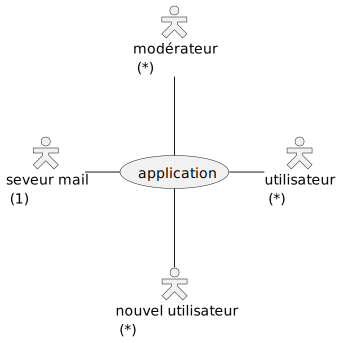
\includegraphics[width=\textwidth]{diag1.pdf}
	    \caption{Diagramme de contexte statique}
	    \label{fig:diag1}
	\end{figure}
	
	
	\chapter{Diagramme des cas d'utilisations}
	\section{Premier diagramme des cas d'utilisations}
	\begin{figure}[H]
	    \centering
	    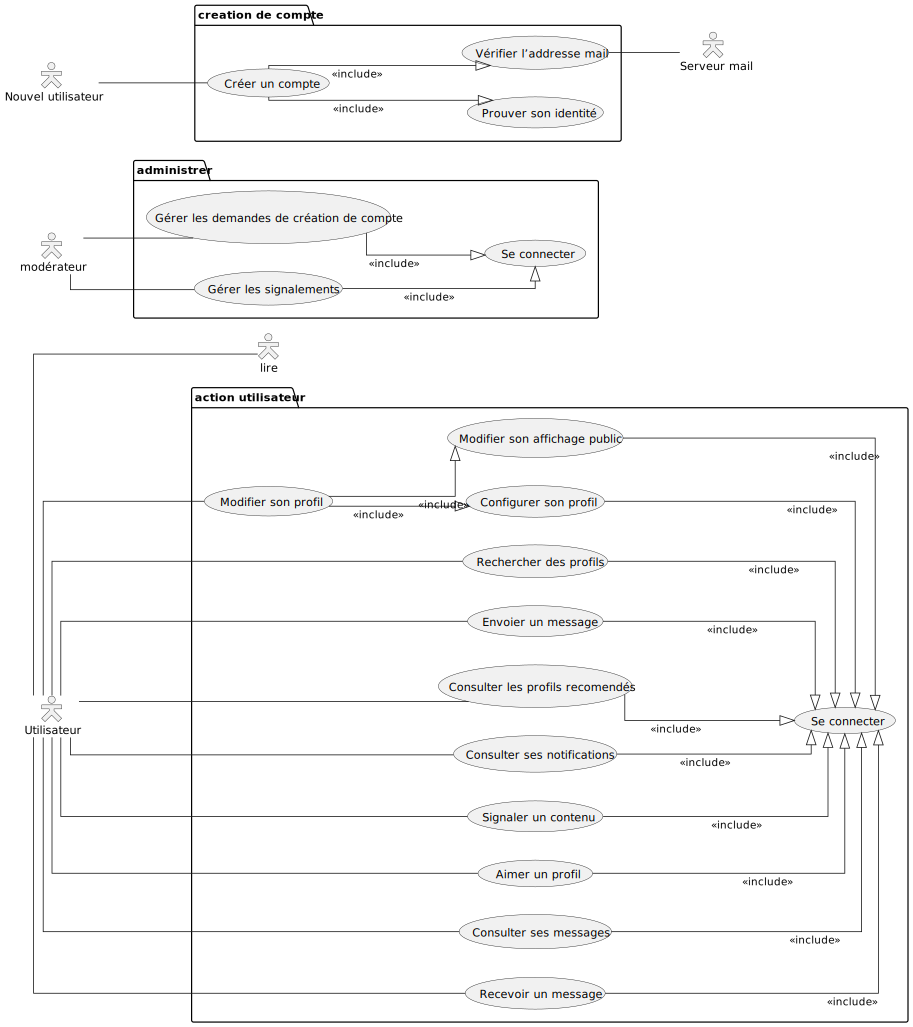
\includegraphics[width=\textwidth]{diag2.pdf}
	    \caption{Diagramme des cas d'utilisations}
	    \label{fig:diag2}
	\end{figure}
	
	\newpage
	
	\section{Description du cas d’utilisation 1 : Créer un compte}
	\subsection{Sommaire d’identification }
	Titre : Créer un compte\\
	Résumé : Ce cas permet à un utilisateur non inscrit de se créer un compte avec un pseudo, une adresse mail, un mot de passe et une pièce d’identité sur l’application. L’inscription est validée après le feu vert du modérateur.\\
	Date de création : 14/10/2025\\
	Acteurs concernés : Utilisateur (non inscrit), modérateur\\
	Responsable : SCHMITT Martin\\
	Auteur : SCHMITT Martin
	
	\subsection{Besoins en IHM }
	Un Téléphone ou ordinateur
	
	\subsection{Contraintes non fonctionnelles}
	Temps de réponse : Aucune latence ne doit être plus longue que 10 millisecondes dans le cadre où la connexion de l’utilisateur est optimale.\\
	Fiabilité : Le système doit vérifier si l’adresse mail est valide.\\
	Disponibilité : Les nouveaux utilisateurs doivent pouvoir s’inscrire quand ils le veulent.
	
	
	\subsection{Descriptions des scénarios}
	1. L’utilisateur se connecte à l’URL.\\
	2. L’application propose la page inscription ou connexion.\\
	3. L’utilisateur choisit la page d’inscription.\\
	4. L’application affiche la page d’inscription.\\
	5. L’utilisateur choisit un pseudo.\\
	6. L’application vérifie le pseudo.\\
	7. L’application valide le pseudo.\\
	8. L’utilisateur choisit une adresse mail.\\
	9. L’application vérifie l’adresse mail.\\
	10. L’application valide l’adresse mail.\\
	11. L’utilisateur choisit un mot de passe.\\
	12. L’application vérifie le mot de passe.\\
	13. L’application valide le mot de passe.\\
	14. L’utilisateur transmet un document d’identité.\\
	15. L’application envoie la demande d’inscription au modérateur.\\
	16. Le modérateur valide la demande.\\
	17. L’application indique que l’inscription est validée et terminée.\\
	
	Description du scénario exceptionnel : Le modérateur invalide la demande.
	Cet enchaînement démarre au point 15 du scénario principal.\\
	16. L’application indique que l’inscription est refusée et doit être recommencée.\\
	
	Description du scénario alternatif : L’application constate que le pseudo n’est pas valide.
	Cet enchaînement démarre au point 6 du scénario principal.
	Cet enchaînement se répète jusqu’à ce que le choix de pseudo soit valide.\\
	7. L’application demande un nouveau pseudo.\\
	8. L’utilisateur choisit un nouveau pseudo.\\
	9. L’application vérifie le nouveau pseudo.\\
	Le scénario nominal reprend au point 7\\
	
	Description du scénario alternatif : L’application constate que l’adresse mail n’est pas valide.
	Cet enchaînement démarre au point 9 du scénario principal.
	Cet enchaînement se répète jusqu’à ce que l'adresse mail soit valide.\\
	10. L’application demande une nouvelle adresse mail.\\
	11. L’utilisateur choisit une nouvelle adresse mail.\\
	12. L’application vérifie la nouvelle adresse mail.\\
	Le scénario nominal reprend au point 10\\
	
	Description du scénario alternatif : L’application constate que le mot de passe n’est pas valide.
	Cet enchaînement démarre au point 12 du scénario principal.
	Cet enchaînement se répète jusqu’à ce que le mot de passe soit valide.\\
	13. L’application demande un nouveau mot de passe.\\
	14. L’utilisateur choisit un nouveau mot de passe.\\
	15. L’application vérifie le nouveau mot de passe.\\
	Le scénario nominal reprend au point 13
	
	\begin{figure}[H]
	    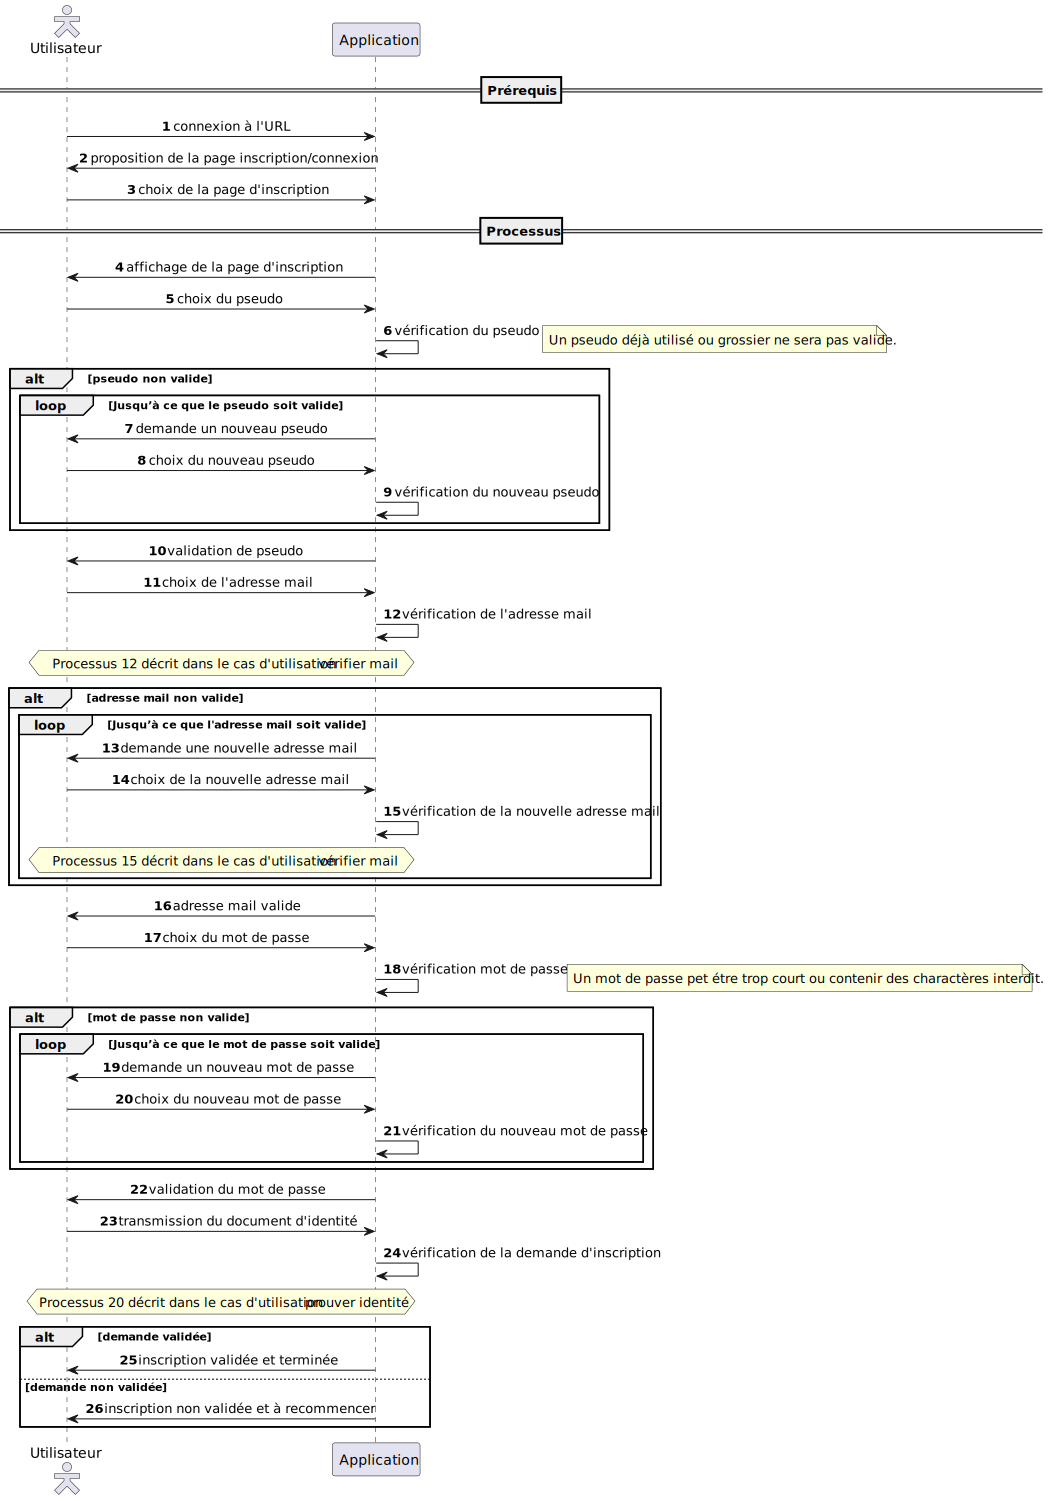
\includegraphics[width=\textwidth]{diag3.pdf}
	    \caption{Diagramme cas d'utilisation 1}
	    \label{fig:diag3}
	\end{figure}
	
	\newpage
	
	\section{Description du cas d’utilisation 2 : Vérifier l’adresse mail}
	\subsection{Sommaire d’identification }
	Titre : Vérifier l’adresse mail\\ 
	Résumé : Ce cas permet à un utilisateur tentant de s’inscrire de pouvoir valider que l’adresse mail qu’il a donnée est valide et bien la sienne, en la validant depuis sa boîte mail personnelle.\\
	Date de création : 15/10/2025\\
	Acteurs concernés : Utilisateur (non inscrit), serveur mail\\
	Responsable : SCHMITT Martin\\
	Auteur : SCHMITT Martin
	
	\subsection{Besoins en IHM }
	Un Téléphone ou ordinateur
	
	\subsection{Contraintes non fonctionnelles}
	Temps de réponse : Le mail doit être reçu dans les plus brefs délais par l’utilisateur. Au bout d’un certain temps, l’utilisateur peut demander à recevoir un nouveau mail.\\
	Fiabilité : Le lien de validation doit être envoyé à la bonne adresse mail.\\
	Disponibilité : Les nouveaux utilisateurs doivent pouvoir recevoir le mail quand ils le veulent.
	
	\subsection{Descriptions des scénarios}
	1. L’utilisateur réalise une inscription.\\
	2. L’utilisateur renseigne une adresse mail.\\
	3. L’application vérifie que l’adresse mail existe et est valide.\\
	4. L’application demande au serveur mail d’envoyer un mail de confirmation.\\
	5. Le serveur mail envoie un mail à l’utilisateur.\\
	6. L’utilisateur consulte sa boîte mail.\\
	7. L’utilisateur valide le mail auprès du serveur mail.\\
	8. Le serveur mail confirme la validation du mail à l’application.\\
	9. L’application valide l’adresse mail utilisée.\\
	10. L’application confirme la validation du mail à l’utilisateur.\\
	
	Description du scénario exceptionnel : L’application invalide l’adresse mail.
	Cet enchaînement démarre au point 3 du scénario principal.\\
	4. L'application prévient l'utilisateur que l'adresse mail n'est pas valide\\
	
	Description du scénario alternatif : L’utilisateur constate que le mail n’est pas reçu.
	Cet enchaînement démarre au point 6 du scénario principal.
	Cet enchaînement se répète jusqu’à ce que le mail soit reçu.\\
	7. L’utilisateur demande au serveur mail un renvoi du mail.\\
	8. Le serveur mail renvoie un mail de confirmation.\\
	9. L’utilisateur consulte la boîte mail.\\
	Le scénario nominal reprend au point 7
	
	\begin{figure}[H]
	    \centering
	    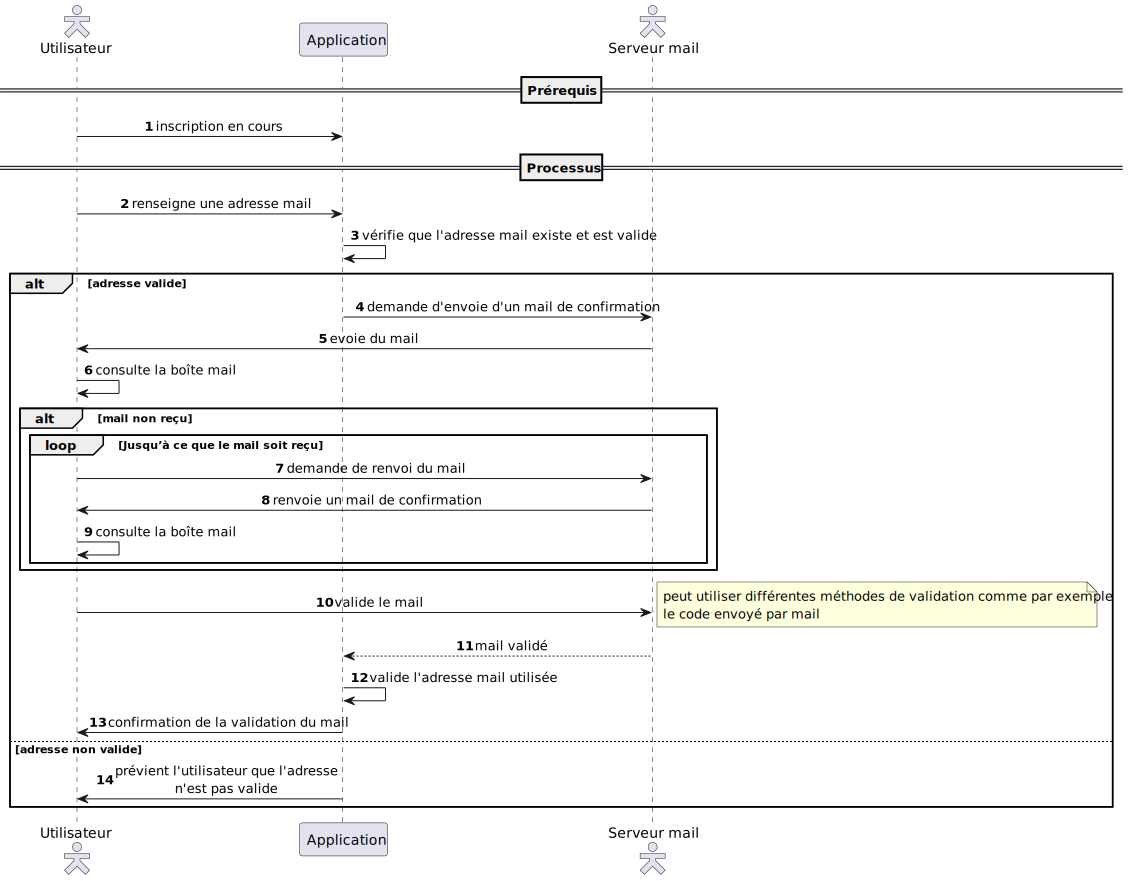
\includegraphics[width=\textwidth]{diag4.pdf}
	    \caption{Diagramme cas d'utilisation 2}
	    \label{fig:diag4}
	\end{figure}
	
	\newpage
	
	\section{Description du cas d’utilisation 3 : Prouver son identité}
	\subsection{Sommaire d’identification }
	Titre : Prouver son identité\\
	Résumé : Ce cas permet à l'utilisateur tentant de s’inscrire de pouvoir envoyer un document afin de vérifier et faire valider son identité par le modérateur.\\
	Date de création : 15/10/2025\\
	Acteurs concernés : Utilisateur (non inscrit)\\
	Responsable : SCHMITT Martin\\
	Auteur : SCHMITT Martin
	
	\subsection{Besoins en IHM }
	Un Téléphone ou ordinateur
	
	\subsection{Contraintes non fonctionnelles}
	Temps de réponse : Le modérateur doit pouvoir valider (ou non) l'identité le plus vite possible.\\
	Fiabilité : La personne validée est bien celle qui a transmis les papiers d'identité.\\
	Disponibilité : Les utilisateurs doivent pouvoir transmettre les documents d'identité quand ils le veulent.\\
	Confidentialité : Le modérateur ne doit pas conservé les données personnelles des utilisateurs et ne doit pas les divulgués
	
	\subsection{Descriptions des scénarios}
	1. L’utilisateur réalise une inscription.\\
	2. L’utilisateur envoie ses papiers d’identité.\\
	3. L’application lance le processus de vérification d’identité.\\
	4. L’application valide la demande.\\
	5. L’application crée le compte.\\
	6. L’application notifie l’utilisateur de la validation.\\
	
	Description du scénario exceptionnel : L’application invalide la demande.
	Cet enchaînement démarre au point 4 du scénario principal.\\
	5. L’application notifie l’utilisateur du refus et de la justification.
	
	\begin{figure}[H]
	    \centering
	    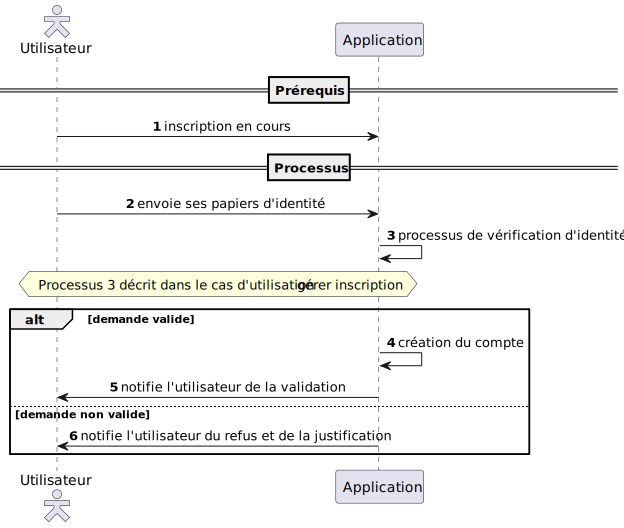
\includegraphics[width=\textwidth]{diag5.pdf}
	    \caption{Diagramme cas d'utilisation 3}
	    \label{fig:diag5}
	\end{figure}
	
	\newpage
	
	\section{Description du cas d’utilisation 4 : Gérer les signalements}
	\subsection{Sommaire d’identification }
	Titre : Gérer les signalements\\
	Résumé : Ce cas permet au modérateur de gérer un signalement.\\
	Date de création : 15/10/2025\\
	Acteurs concernés : modérateur\\
	Responsable : SCHMITT Martin\\
	Auteur : SCHMITT Martin
	
	\subsection{Besoins en IHM }
	Un Téléphone ou ordinateur
	
	\subsection{Contraintes non fonctionnelles}
	Temps de réponse : Le modérateur doit pouvoir gérer le signalement le plus vite possible.\\
	Fiabilité : Le signalement est bien légitime.\\
	Disponibilité : Tout le temps, car les utilisateurs peuvent signaler quand ils le veulent.\\
	Confidentialité : Le modérateur ne doit pas conservé les données personnelles des utilisateurs et ne doit pas les divulgués
	
	\subsection{Descriptions des scénarios}
	1. L’utilisateur signale un contenu douteux.\\
	2. L’application prévient le modérateur du signalement.\\
	3. Le modérateur commence le processus de vérification.\\
	4. L’application envoie les informations du signalement au modérateur.\\
	5. Le modérateur vérifie le signalement.\\
	6. Le modérateur juge le contenu non problématique.\\
	7. Le modérateur annule le signalement.\\
	8. L’application demande une justification.\\
	9. Le modérateur fournit une justification.\\
	10. L’application prévient l’utilisateur ayant émis le signalement et transmet la justification.\\
	11. Le modérateur termine le processus de vérification.\\
	
	Description du scénario alternatif : Le modérateur juge le contenu inapproprié.
	Cet enchaînement démarre au point 6 du scénario principal.\\
	7. Le modérateur bloque la personne signalée.\\
	8. L’application demande une justification.\\
	9. Le modérateur fournit une justification.\\
	10. L’application prévient l’utilisateur signalé et transmet la justification.\\
	Le scénario nominal reprend au point 11
	
	\begin{figure}[H]
	    \centering
	    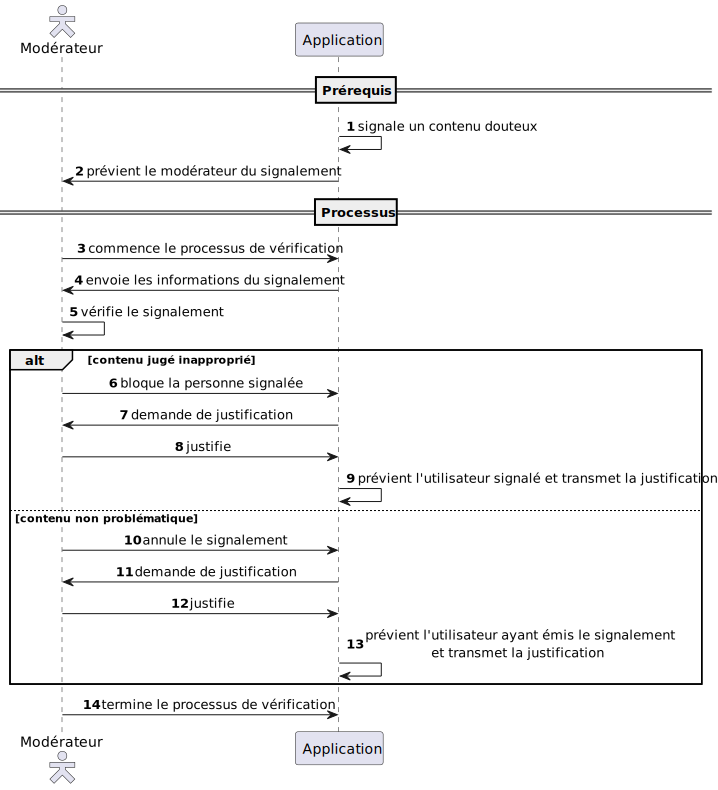
\includegraphics[width=\textwidth]{diag6.pdf}
	    \caption{Diagramme cas d'utilisation 4}
	    \label{fig:diag6}
	\end{figure}
	
	\newpage
	
	\section{Description du cas d’utilisation 5 : Gérer les demande de création de compte}
	\subsection{Sommaire d’identification }
	Titre : Gérer les demande de création de compte\\
	Résumé : Ce cas permet au modérateur de vérifier si l'inscription d'un utilisateur est valide.\\
	Date de création : 15/10/2025\\
	Acteurs concernés : Application, modérateur\\
	Responsable : SCHMITT Martin
	Auteur : SCHMITT Martin
	
	\subsection{Besoins en IHM }
	Un Téléphone ou ordinateur
	
	\subsection{Contraintes non fonctionnelles}
	Temps de réponse : Le modérateur doit pouvoir valider (ou non) l'identité le plus vite possible.\\
	Fiabilité : L'identité fournie par l'utilisateur est bien valide, et l'identité fournie n'est pas déjà utilisée.\\
	Disponibilité : Tout le temps, car les utilisateurs peuvent transmettre les documents d'identité quand ils le veulent.\\
	Confidentialité : Le modérateur ne doit pas conservé les données personnelles des utilisateurs et ne doit pas les divulgués
	
	\subsection{Descriptions des scénarios}
	1. L’application notifie une demande d’inscription au modérateur.\\
	2. Le modérateur commence le processus de vérification.\\
	3. L’application envoie des documents d’identité au modérateur.\\
	4. Le modérateur vérifie si l’identité est déjà associée à un compte.\\
	5. Le modérateur vérifie si l’individu a un âge légal.\\
	6. Le modérateur vérifie si l’identité n’est pas blacklistée des sites de rencontre.\\
	7. Le modérateur vérifie si l’identité existe réellement.\\
	8. le modérateur valide l’inscription.\\
	
	Description du scénario exceptionnel : l'un des cas vérifié n'est pas valide
	Cet enchaînement démarre au point 7 du scénario principal.\\
	8. le modérateur refuse l’inscription.
	
	\begin{figure}[H]
	    \centering
	    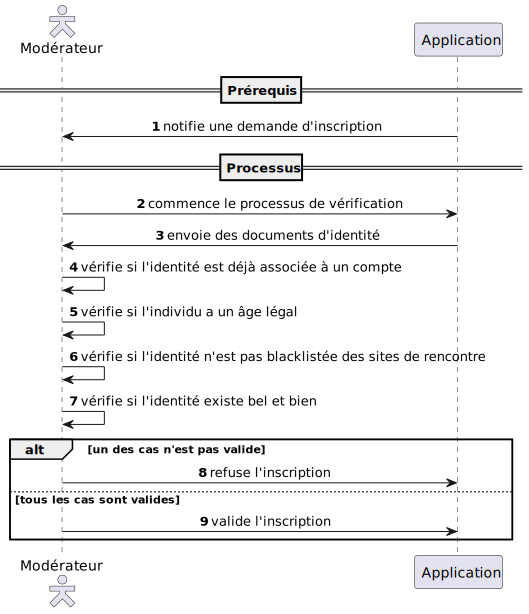
\includegraphics[width=\textwidth]{diag7.pdf}
	    \caption{Diagramme cas d'utilisation 5}
	    \label{fig:diag7}
	\end{figure}
	
	\newpage
	
	\section{Description du cas d’utilisation 6 : Se connecter}
	\subsection{Sommaire d’identification }
	Titre : Se connecter\\
	Résumé : Ce cas permet à l’utilisateur de se connecter\\
	Date de création : 18/10/2025\\
	Acteurs concernés : Utilisateur, application\\
	Responsable : SIGNORINO-GELO Matteo\\
	Auteur : SIGNORINO-GELO Matteo

	
	\subsection{Besoins en IHM }
	Un Téléphone ou ordinateur
	
	\subsection{Contraintes non fonctionnelles}
	Temps de réponse : Aucune latence ne doit être plus longue que 10 millisecondes dans le cadre où la connexion de l’utilisateur est optimale.\\
	Fiabilité : Les connexions ne doivent pas échouer à cause de l'application\\
	Disponibilité : Les utilisateurs doivent pouvoir se connecter tout le temps.
	
	\subsection{Descriptions des scénarios}
	1. L'utilisateur accède à la page de connexion\\
	2. L'application demande à l'utilisateur d'entrer ses identifiants de connexions\\
	3. l'utilisateur entre ses identifiants de connexions\\
	4. L'application vérifie les informations reçus\\
	
	Description du scénario alternatif :\\
	5. L'application invalide les informations\\
	6. L'utilisateur renseigne les bonnes informations\\
	7. L'application vérifie les informations reçus\\
	
	8.L'application valide les informations\\
	9. L'application confirme l'authentification de l'utilisateur\\
	10. L'application redirige l'utilisateur vers la page d'accueil\\
	
	
	\begin{figure}[H]
	    \centering
	    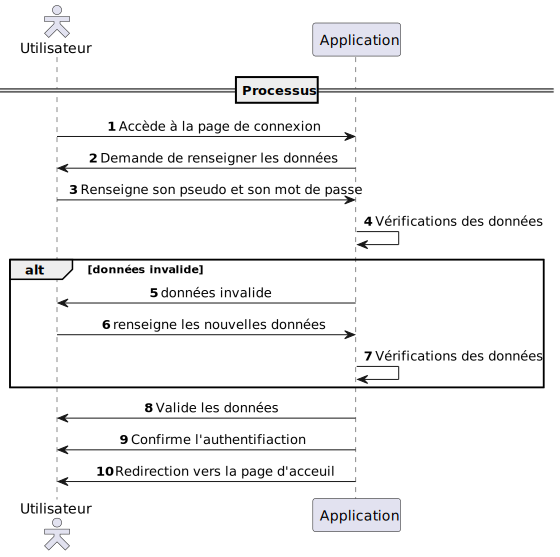
\includegraphics[width=\textwidth]{diag8.pdf}
	    \caption{Diagramme cas d'utilisation 6}
	    \label{fig:diag8}
	\end{figure}
	
	\newpage
	
	\section{Description du cas d’utilisation 7 : Modifier son profil}
	\subsection{Sommaire d’identification }
	Titre : Modifier son profil\\
	Résumé : Ce cas permet à l’utilisateur de modifier son profil public\\
	Date de création : 18/10/2025\\
	Acteurs concernés : Utilisateur, application\\
	Responsable : HENRY Romaric\\
	Auteur : HENRY Romaric

	
	\subsection{Besoins en IHM }
	Un Téléphone ou ordinateur
	
	\subsection{Contraintes non fonctionnelles}
	Temps de réponse : Aucune latence ne doit être plus longue que 10 millisecondes dans le cadre où la connexion de l’utilisateur est optimale.\\
	Fiabilité : Les modifications doivent s'enregistrer sans aucune problématiques\\
	Disponibilité : Les utilisateurs doivent pouvoir modifier leur profil tout le temps.
	
	\subsection{Descriptions des scénarios}
	Requière d'être connecter.\\
	Si l'utilisateur veut configurer son profil, se référer au cas d'utilisation du même nom.\\
	Si l'utilisateur veut modifier l'affichage de son profil affichage public, se référer au cas d'utilisation du même nom.\\
	
	\begin{figure}[H]  
	    \centering
	    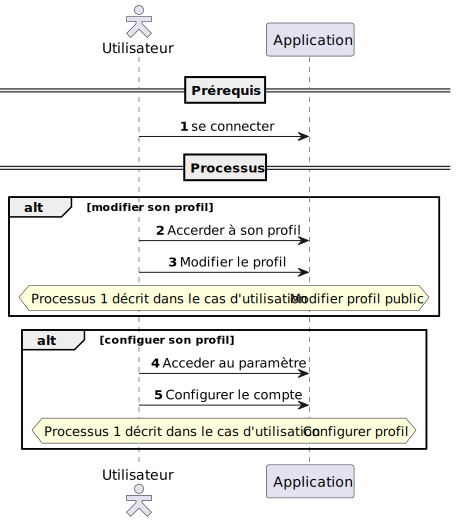
\includegraphics[width=\textwidth]{diag9.pdf}
	    \caption{Diagramme cas d'utilisation 7}
	    \label{fig:diag9}
	\end{figure}
	
	\newpage
	
	\section{Description du cas d’utilisation 8 : Configurer son profil}
	\subsection{Sommaire d’identification }
	Titre : Configurer son profil\\
	Résumé : Ce cas permet à l’utilisateur de configurer son profil public, comme les paramètres de notifications, les critères que doivent valider les autres utilisateurs pour pouvoir consulter le profil de l'utilisateur, mais aussi les critères des profils qu'il lui seront recommandés.\\
	Date de création : 18/10/2025\\
	Acteurs concernés : Utilisateur, application\\
	Responsable : HENRY Romaric\\
	Auteur : HENRY Romaric
	
	\subsection{Besoins en IHM }
	Un Téléphone ou ordinateur
	
	\subsection{Contraintes non fonctionnelles}
	Temps de réponse : Aucune latence ne doit être plus longue que 10 millisecondes dans le cadre où la connexion de l’utilisateur est optimale.\\
	Fiabilité : Les modifications doivent s'enregistrer sans aucune problématiques\\
	Disponibilité : Les utilisateurs doivent pouvoir configurer leur profil tout le temps.
	
	\subsection{Descriptions des scénarios}
	Prérequis : être connecté\\
	Processus : \\
	1. L'utilisateur sélectionne le menu de configuration du profil\\
	
	Description du scénario alternatif de modification des paramètres de notifications: \\
	2. L'utilisateur sélectionne le menu des paramètres de notifications\\
	Option mail :\\
	3. L'utilisateur sélectionne ou désélectionne l'option de notification doublé par mail\\
	Option application :\\
	4. L'utilisateur sélectionne ou désélectionne l'option de notification uniquement sur application\\
	
	Description du scénario alternatif des paramètres des profils recommandés\\
	5. L'utilisateur sélectionne le menu profil recommandé\\
	6. L'utilisateur ajoute ou enlève des critères de sélections\\
	
	Description du scénario alternatif des paramètres des profils recommandés\\
	7. L'utilisateur sélectionne le menu visibilité du profil\\
	8. L'utilisateur ajoute ou enlève des critères de sélections\\
	
	L'utilisateur confirme ses modifications et l'application lui rend compte de leurs prises en compte.
	
	\begin{figure}[H]
	    \centering
	    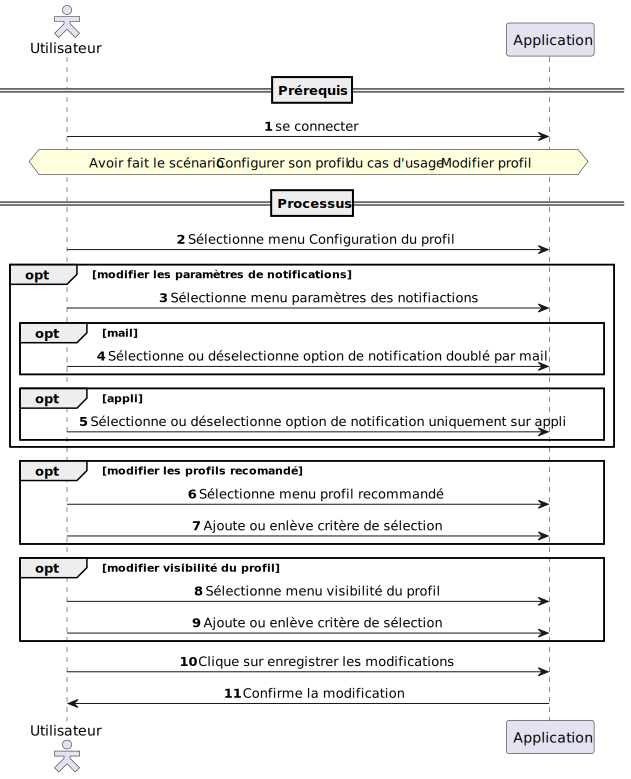
\includegraphics[width=\textwidth]{diag10.pdf}
	    \caption{Diagramme cas d'utilisations 8}
	    \label{fig:diag10}
	\end{figure}
	
	\newpage
	
	\section{Description du cas d’utilisation 9 : Modifier son affichage public}
	\subsection{Sommaire d’identification }
	Titre : Modifier son affichage public\\
	Résumé : Ce cas permet à l’utilisateur de modifier son profil public, c'est-à-dire ce que voient les autres utilisateurs\\
	Date de création : 18/10/2025\\
	Acteurs concernés : Utilisateur, application\\
	Responsable : HENRY Romaric\\
	Auteur : HENRY Romaric
	
	\subsection{Besoins en IHM }
	Un Téléphone ou ordinateur
	
	\subsection{Contraintes non fonctionnelles}
	Temps de réponse : Aucune latence ne doit être plus longue que 10 millisecondes dans le cadre où la connexion de l’utilisateur est optimale.\\
	Fiabilité : Les modifications doivent s'enregistrer sans aucune problématiques\\
	Disponibilité : Les utilisateurs doivent pouvoir modifier leur profil tout le temps.
	
	
	\subsection{Descriptions des scénarios}
	L'utilisateur une fois connecté et après avoir réalisé le cas d'utilisation "modifier son profil" arrive sur la page de modification de son profil public.
	Il peut cliquer sur chaque champ pour le modifier. Les champs sont l'âge, le pseudo, la ville, le genre, les centre d'intérêts, la biographie et les médias. Le choix de la ville ce fait parmi une sélection. Le genre, le pseudo, la ville, les centre d'intérêts et la biographie, sont des zones de textes, que l'utilisateur peut remplir "librement". L'utilisateur peut également ajouter des médias en cliquant sur l'option éponyme. Pour les "supprimer" il doit faire un appuie long pour les sélectionner puis cliquer sur l'option supprimer. Pour que les changements soient pris en compte, il est impératif de cliquer sur le bouton "enregistrer les modifications", l'application confirmera les changements.
	
	\begin{figure}[H]
	    \centering
	    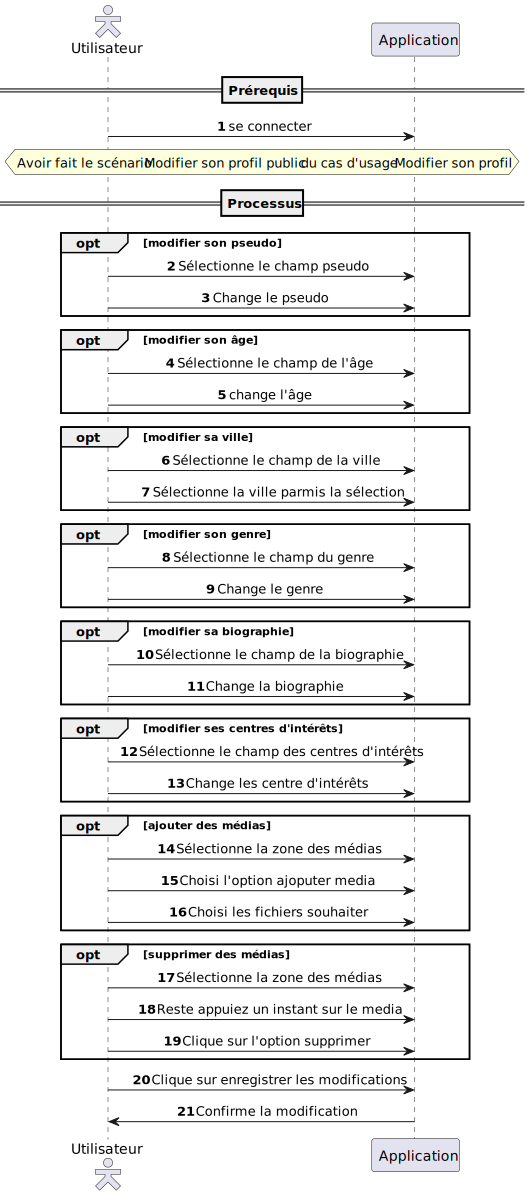
\includegraphics[scale=0.7]{diag11.pdf}
	    \caption{Diagramme cas d'utilisation 9}
	    \label{fig:diag11}
	\end{figure}
	
	\newpage
	
	\section{Description du cas d’utilisation 10 : Consulter ses notifications}
	\subsection{Sommaire d’identification }
	Titre : Consulter ses notifications\\
	Résumé : Ce cas permet à l'utilisateur de consulter ses notifications. Si il l'a accepté il peut aussi recevoir un mail\\
	Date de création : 16/10/2025\\
	Acteurs concernés : Utilisateur, serveur mail\\
	Responsable : SCHMITT Martin\\
	Auteur : SCHMITT Martin
	
	\subsection{Besoins en IHM }
	Un Téléphone ou ordinateur
	
	\subsection{Contraintes non fonctionnelles}
	Temps de réponse : Aucune latence ne doit être plus longue que 10 millisecondes dans le cadre où la connexion de l’utilisateur est optimale.\\
	Fiabilité : L'utilisateur doit avoir validé la réception des notifications (modifier profil). Dans le cas où il ne l’a pas fait, il n’en reçoit pas.\\
	Disponibilité : Les utilisateurs doivent pouvoir consulter leurs notifications tout le temps.
	
	\subsection{Descriptions des scénarios}
	1. L’application reçoit une notification.\\
	2. L’application enregistre la notification.\\
	3. L’application ping l’utilisateur.\\
	4. L’application vérifie si l’option d’envoi de mail est activée.\\
	5. L’utilisateur se connecte à l’application.\\
	6. L’utilisateur vérifie les notifications.\\
	7. L’utilisateur interagit avec les notifications.\\
	8. L’utilisateur supprime les notifications.\\
	
	Description du scénario alternatif : l'utilisateur a activer l'option de l'envoie de mail
	Cet enchaînement démarre au point 4 du scénario principal.\\
	5. Le serveur mail envoie un mail à l’utilisateur.\\
	6. L’utilisateur reçoit le mail.\\
	7. L’utilisateur consulte sa boîte mail.\\
	Le scénario nominal reprend au point 5
	
	\begin{figure}[H]
	    \centering
	    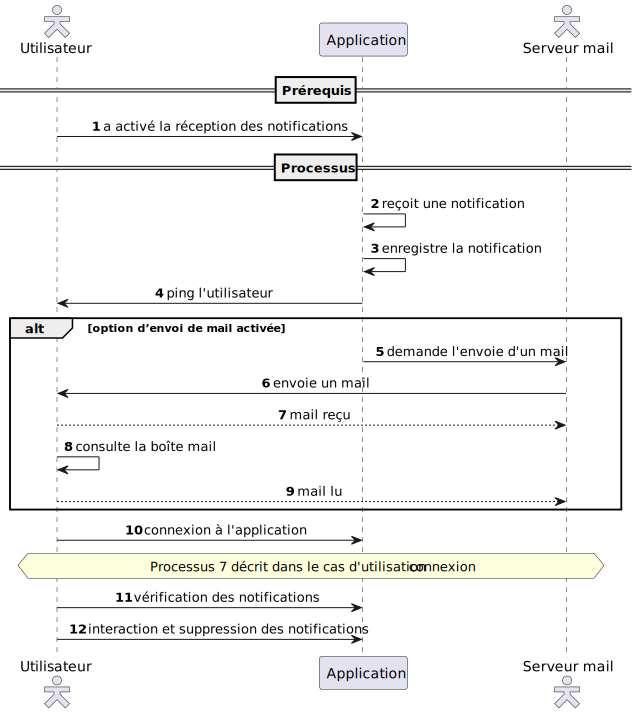
\includegraphics[width=\textwidth]{diag12.pdf}
	    \caption{Diagramme cas d'utilisation 10}
	    \label{fig:diag12}
	\end{figure}
	
	\newpage
	
	\section{Description du cas d’utilisation 11 : Consulter les profils recommandé}
	\subsection{Sommaire d’identification }
	Titre : Consulter les profils recommandé\\
	Résumé : Ce cas permet à l’utilisateur de regarder les profils que l'application lui recommande sur la base de son profil\\
	Date de création : 18/10/2025\\
	Acteurs concernés : Utilisateur, application\\
	Responsable : SIGNORINO-GELO Matteo\\
	Auteur : SIGNORINO-GELO Matteo
	
	\subsection{Besoins en IHM }
	Un Téléphone ou ordinateur
	
	\subsection{Contraintes non fonctionnelles}
	Temps de réponse : Aucune latence ne doit être plus longue que 10 millisecondes dans le cadre où la connexion de l’utilisateur est optimale.\\
	Fiabilité : La consultation des recommandation doit toujours fonctionner\\
	Disponibilité : Les utilisateurs doivent pouvoir consulter ses recommandation à n'importe qu'elle moment.
	
	\subsection{Descriptions des scénarios}
	Prérequis :\\
	1. L'utilisateur c'est connecté à l'application\\
	
	Processus :\\
	2. L'utilisateur sélectionne l'onglet "recommandation de profil"\\
	3. L'application affiche un profil selon les préférences de l'utilisateur\\
	
	Description du scénario alternatif : l'utilisateur n'est pas intéressé\\
	Cet enchaînement démarre au point 3\\
	4. L'utilisateur choisit l'option "voir le profil suivant"\\
	5. L'application affiche un autre profil selon les préférences de l'utilisateur\\
	
	Option : L'utilisateur veut plus de détails sur le profil affiché\\
	6. L'utilisateur clique sur le profil\\
	7. L'application affiche le profil en détail\\
	
	Description du scénario alternatif : L'utilisateur est intéressé par le profil\\
	Cet enchaînement démarre au point 3\\
	8. L'utilisateur clique sur l'option "intéressé"\\
	9. L'application confirme la décision à l'utilisateur\\
	10. L'application gère l'envoie de notification au profil concerné
	
	\begin{figure}[H]
	    \centering
	    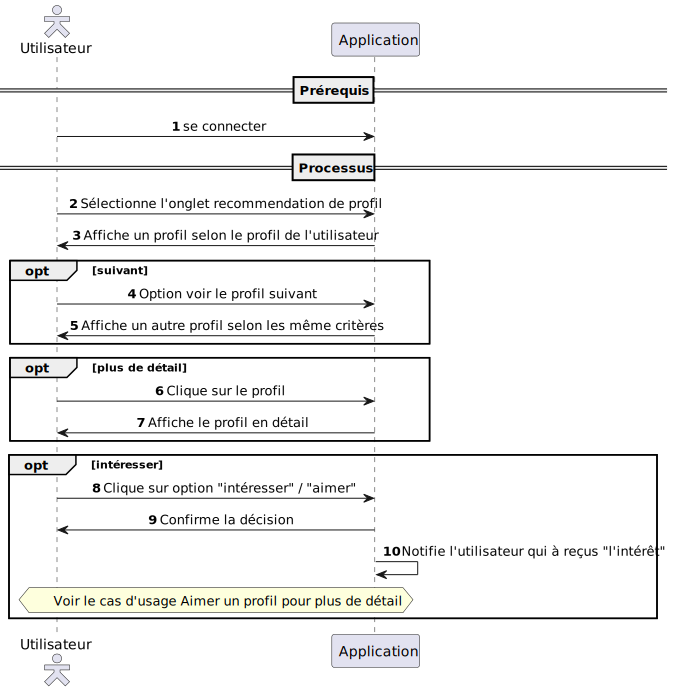
\includegraphics[width=\textwidth]{diag13.pdf}
	    \caption{Diagramme cas d'utilisation 11}
	    \label{fig:diag13}
	\end{figure}
	
	\newpage
	
	\section{Description du cas d’utilisation 12 : Rechercher des profils}
	\subsection{Sommaire d’identification }
	Titre : Rechercher des profils\\
	Résumé : Ce cas permet à l’utilisateur de rechercher un profil\\
	Date de création : 18/10/2025\\
	Acteurs concernés : Utilisateur, application\\
	Responsable : SIGNORINO-GELO Matteo\\
	Auteur : SIGNORINO-GELO Matteo
	
	\subsection{Besoins en IHM }
	Un Téléphone ou ordinateur
	
	\subsection{Contraintes non fonctionnelles}
	Temps de réponse : Aucune latence ne doit être plus longue que 10 millisecondes dans le cadre où la connexion de l’utilisateur est optimale.\\
	Fiabilité : La recherche doit toujours fonctionner\\
	Disponibilité : Les utilisateurs doivent pouvoir rechercher un profil à n'importe qu'elle moment.
	
	\subsection{Descriptions des scénarios}
	Prérequis : \\
	1. L'utilisateur c'est connecté à l'application\\
	
	Processus :\\
	2. L'utilisateur sélectionne l'onglet "rechercher profil"\\
	3. L'application affiche la page correspondante\\
	
	Option : Distance de la recherche\\
	4. L'utilisateur sélectionne la distance maximal voulue pour la recherche de profil\\
	
	Option : Tranche d'age voulu\\
	5. L'utilisateur sélectionne la tranche d'age voulu pour la recherche de profil\\
	
	Option : Genre voulue\\
	6. L'utilisateur choisit le genre voulue pour la recherche de profil\\
	
	Option : Centre d'intérêts\\
	7. L'utilisateur choisit parmi une sélection de centre d'intérêt celui ou ceux qui l'intéresse\\
	
	Fin des options, reprise du scénario\\
	8. L'utilisateur valide ses choix\\
	9. L'application affiche les profiles correspondant
	
	\begin{figure}[H]
	    \centering
	    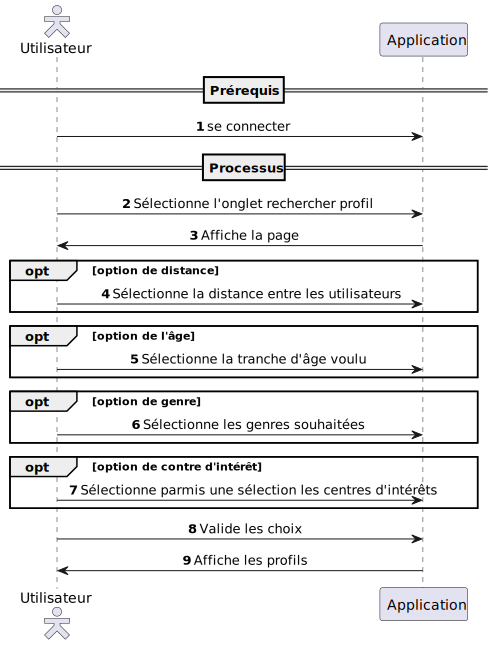
\includegraphics[width=\textwidth]{diag14.pdf}
	    \caption{Diagramme cas d'utilisations 12}
	    \label{fig:diag14}
	\end{figure}
	
	\newpage
	
	\section{Description du cas d’utilisation 13 : Aimer un profil}
	\subsection{Sommaire d’identification }
	Titre : Aimer un profil\\
	Résumé : Ce cas permet à l’utilisateur dire qu'un profil lui plaît\\
	Date de création : 18/10/2025\\
	Acteurs concernés : Utilisateur, application\\
	Responsable : SIGNORINO-GELO Matteo\\
	Auteur : SIGNORINO-GELO Matteo
	
	\subsection{Besoins en IHM }
	Un Téléphone ou ordinateur
	
	\subsection{Contraintes non fonctionnelles}
	Temps de réponse : Aucune latence ne doit être plus longue que 10 millisecondes dans le cadre où la connexion de l’utilisateur est optimale.\\
	Fiabilité : le match doit jamais échouer\\
	Disponibilité : Les utilisateurs doivent pouvoir dire qu'un profil les intéressent à n'importe quelle moment.
	
	\subsection{Descriptions des scénarios}
	Prérequis : \\
	1. L'utilisateur c'est connecté à l'application\\
	2. L'utilisateur consulte un produit\\
	
	Processus :\\
	
	Option : Depuis un profil\\
	3. L'utilisateur sélectionne les options du profil\\
	4. L'utilisateur sélectionne l'option "intéressé par le profil"\\
	5. L'utilisateur valide son action\\
	6. L'application gère l'envoie de notification au profil concerné\\
	
	Option :  Depuis l'onglet "recommandation"\\
	7. L'utilisateur sélectionne l'option "intéressé par le profil"\\
	8. L'utilisateur valide son action\\
	9. L'application gère l'envoie de notification au profil concerné\\
	
	\begin{figure}[H]
	    \centering
	    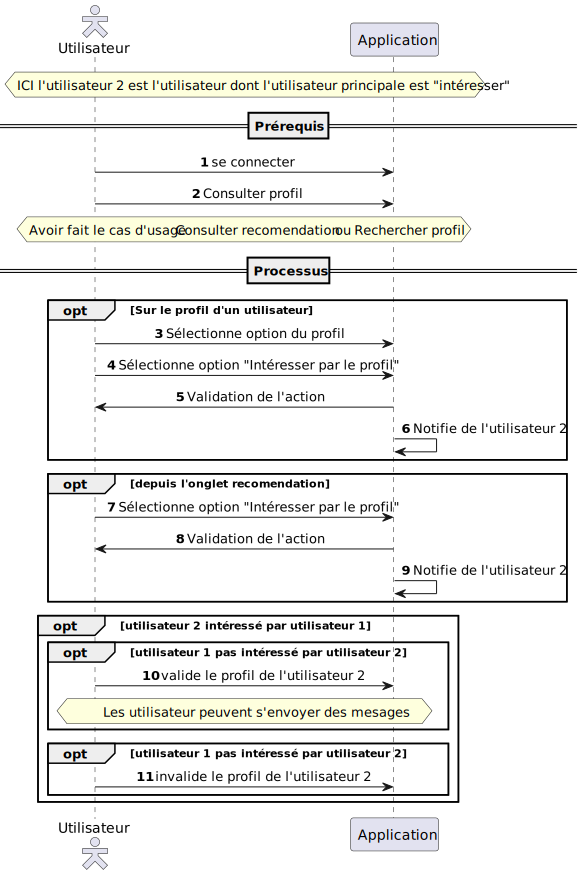
\includegraphics[scale=0.9]{diag15.pdf}
	    \caption{Diagramme cas d'utilisation 13}
	    \label{fig:diag15}
	\end{figure}
	
	\newpage
	
	\section{Description du cas d’utilisation 14 : Consulter ses messages}
	\subsection{Sommaire d’identification }
	Titre : Consulter ses messages\\
	Résumé : Ce cas permet à l’utilisateur de regarder ces messages\\
	Date de création : 18/10/2025\\
	Acteurs concernés : Utilisateur, application\\
	Responsable : SIGNORINO-GELO Matteo\\
	Auteur : SIGNORINO-GELO Matteo
	
	\subsection{Besoins en IHM }
	Un Téléphone ou ordinateur
	
	\subsection{Contraintes non fonctionnelles}
	Temps de réponse : Aucune latence ne doit être plus longue que 10 millisecondes dans le cadre où la connexion de l’utilisateur est optimale.\\
	Fiabilité : l’ouverture d'un messages ne doit jamais échouer\\
	Disponibilité : Les utilisateurs doivent pouvoir consulter leur messages tout le temps.
	
	\subsection{Descriptions des scénarios}
	Processus :\\
	1. L'utilisateur connecté accède à la messagerie\\
	2. L'application affiche les conversations que l'utilisateur possède\\
	3. L'application notifie l'utilisateur des messages non lus\\
	4. L'utilisateur choisit une conversation\\
	5. L'application affiche les messages de cette conversation
	
	\begin{figure}[H]
	    \centering
	    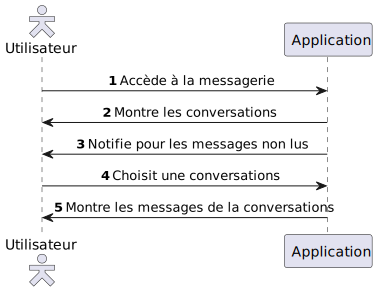
\includegraphics[width=\textwidth]{diag16.pdf}
	    \caption{Diagramme cas d'utilisation 14}
	    \label{fig:diag16}
	\end{figure}
	
	\newpage
	
	\subsection{Description du cas d’utilisation 15 : Envoyer un message}
	\subsection{Sommaire d’identification }
	Titre : Envoyer un message\\
	Résumé : Ce cas permet à l'utilisateur d'envoyer un message. Un premier message ne peut être envoyé qu'après la validation du profil. La conversation ne peut continuer qu'après le match.\\
	Date de création : 16/10/2025\\
	Acteurs concernés : Utilisateur, application\\
	Responsable : SCHMITT Martin\\
	Auteur : SCHMITT Martin
	
	\subsection{Besoins en IHM }
	Un Téléphone ou ordinateur
	
	\subsection{Contraintes non fonctionnelles}
	Temps de réponse : Aucune latence ne doit être plus longue que 10 millisecondes dans le cadre où la connexion de l’utilisateur est optimale.\\
	Fiabilité : Mis à part un premier message, l’envoi de message ne peut pas être effectué avant qu’il y ait match.\\
	Disponibilité : Les utilisateurs doivent pouvoir envoyer des messages tout le temps.	
	
	\subsection{Descriptions des scénarios}
	1. L’utilisateur valide un profil.\\
	2. L’utilisateur envoie un message.\\
	3. L’application bloque l’envoi de message.\\
	4. L’utilisateur attend une réponse.\\
	5. L’application constate qu’il y a un match.\\
	6. L’application informe l’utilisateur qu’il y a match.\\
	7. L’application débloque l’envoi de message.\\
	Cet enchaînement se répète tant que la conversation dure.\\
	8. L’utilisateur envoie un ou plusieurs messages.\\
	9. L’utilisateur attend une réponse.\\
	
	Description du scénario exceptionnel : L’application constate qu’il n’y a pas de match.\\
	Cet enchaînement démarre au point 4 du scénario principal.\\
	5. L’application informe l’utilisateur qu’il n’y a pas de match.
	
	\begin{figure}[H]
	    \centering
	    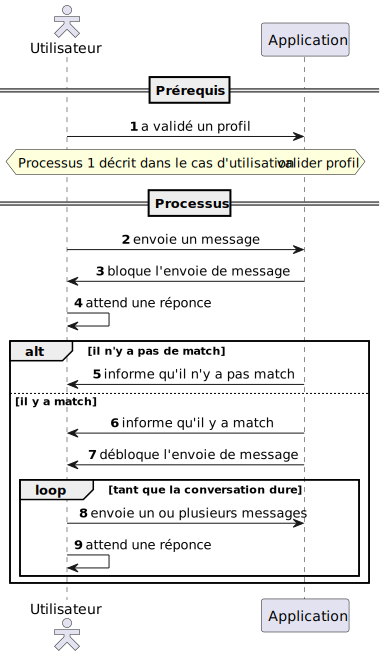
\includegraphics{diag17.pdf}
	    \caption{Diagramme cas d'utilisation 15}
	    \label{fig:diag17}
	\end{figure}
	
	\newpage
	
	\section{Description du cas d’utilisation 16 : Signaler un contenu}
	\subsection{Sommaire d’identification }
	Titre : Signaler un contenu\\
	Résumé : Ce cas permet à l’utilisateur de signaler un contenu\\
	Date de création : 18/10/2025\\
	Acteurs concernés : Utilisateur, application\\
	Responsable : SIGNORINO-GELO Matteo\\
	Auteur : SIGNORINO-GELO Matteo
	
	\subsection{Besoins en IHM }
	Un Téléphone ou ordinateur
	
	\subsection{Contraintes non fonctionnelles}
	Temps de réponse : Aucune latence ne doit être plus longue que 10 millisecondes dans le cadre où la connexion de l’utilisateur est optimale.\\
	Fiabilité : Le signalement doit toujours fonctionner\\
	Disponibilité : Les utilisateurs doivent pouvoir signaler un contenu à n'importe qu'elle moment.
	
	\subsection{Descriptions des scénarios}
	Processus :\\
	
	Description du scénario alternatif : L'utilisateur signale un message :\\
	1. L'utilisateur sélectionne le message souhaité\\
	2. L'application affiche les options sur le message\\
	3. L'utilisateur sélectionne "signaler le message"\\
	4. L'application envoie un message de confirmation\\
	5. L'application envoie le message signalé au modérateur\\
	
	Description du scénario alternatif : l'utilisateur signale un profil\\
	6. L'utilisateur sélectionne le profil souhaité\\
	7. L'utilisateur sélectionne les options du profil\\
	8. L'application montre les options du profil\\
	9. L'utilisateur sélectionne "signaler le profil"\\
	10. L'application envoie un message de confirmation\\
	11. L'application envoie le profil signalé au modérateur\\
	
	Description du scénario alternatif : L'utilisateur signale un contenu (image, photo..):\\
	1. L'utilisateur sélectionne le contenu souhaité\\
	2. L'application affiche les options du contenu\\
	3. L'utilisateur sélectionne "signaler le contenu"\\
	4. L'application envoie un message de confirmation\\
	5. L'application envoie le contenu signalé au modérateur\\
	
	\begin{figure}[H]
	    \centering
	    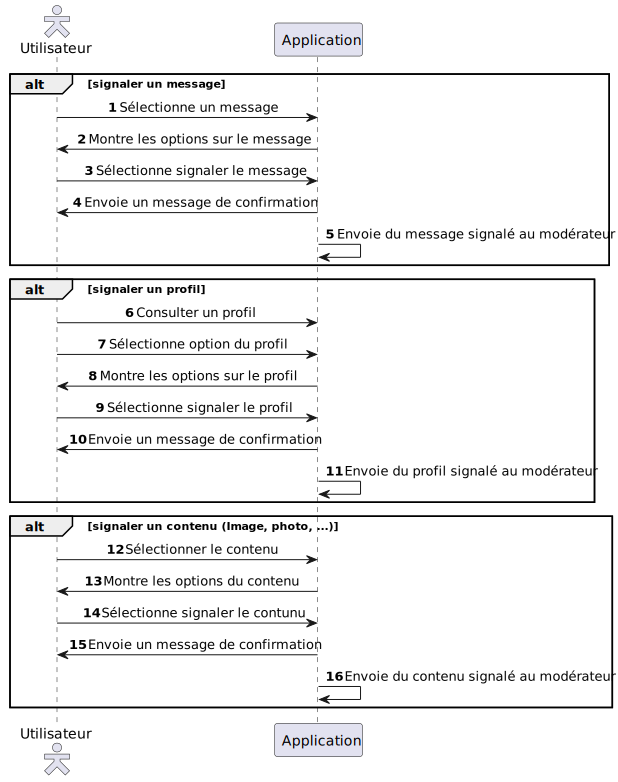
\includegraphics[width=\textwidth]{diag18.pdf}
	    \caption{Diagramme cas d'utilisation 16}
	    \label{fig:diag18}
	\end{figure}
	
	\newpage
	
	\section{Description du cas d’utilisation 17 : Recevoir un message}
	\subsection{Sommaire d’identification }
	Titre : Recevoir un message\\
	Résumé : Ce cas permet à l’utilisateur de recevoir un message\\
	Date de création : 26/11/2025\\
	Acteurs concernés : Utilisateur, application\\
	Responsable : SCHMITT Martin\\
	Auteur : SCHMITT Martin
	
	\subsection{Besoins en IHM }
	Un Téléphone ou ordinateur
	
	\subsection{Contraintes non fonctionnelles}
	Temps de réponse : Aucune latence ne doit être plus longue que 10 millisecondes dans le cadre où la connexion de l’utilisateur est optimale.\\
	Fiabilité : Le message doit toujours être reçus\\
	Disponibilité : Les utilisateurs doivent pouvoir recevoir leur message à n'importe quelle moment
	
	\subsection{Descriptions des scénarios}
	1. L’utilisateur reçoit un message.\\
	2. L'utilisateur consulte le message.\\
	
	Description du scénario alternatif : l’option mail est activée.\\
	Cet enchaînement démarre au point 1 du scénario principal.\\
	2. L’application demande au serveur mail d’envoyer un mail.\\
	3. Le serveur mail envoie un mail à l’utilisateur.\\
	4. L’utilisateur consulte sa boîte mail.\\
	Le scénario nominal reprend au point 2\\
	
	description du scénario exceptionnel : premier message reçu d'un autre utilisateur\\
	Cet enchaînement démarre au point 2 du scénario principal.\\
	3. L’utilisateur peut choisir de matcher.
	
	\begin{figure}[H]
		\centering
		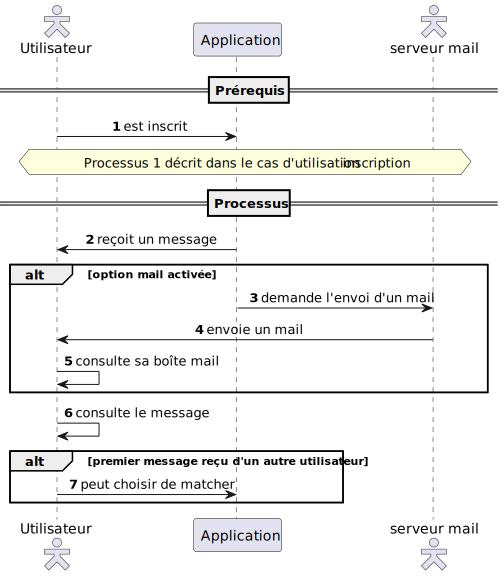
\includegraphics[width=\textwidth]{diag21.pdf}
		\caption{Diagramme cas d'utilisation 17}
		\label{fig:diag31}
	\end{figure}
	
	
	
	
	
	\chapter{Modèle de donné}
	\section{Diagramme d'état d'un compte}
	\begin{figure}[H]
	    \centering
	    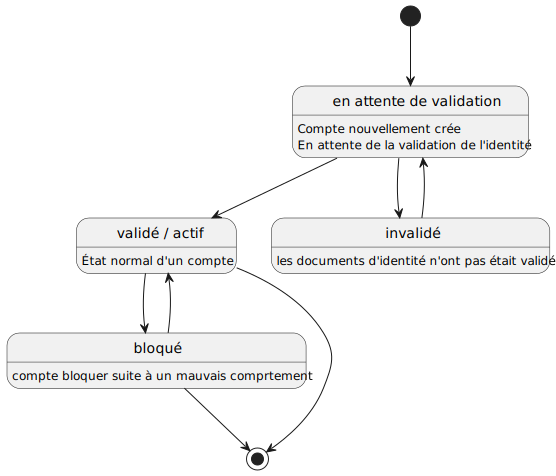
\includegraphics[width=\textwidth]{diag19.pdf}
	    \caption{Diagramme d'état d'un compte}
	    \label{fig:diag19}
	\end{figure}
	
	
	\section{Diagramme de classe}
	\begin{figure}[H]
	    \centering
	    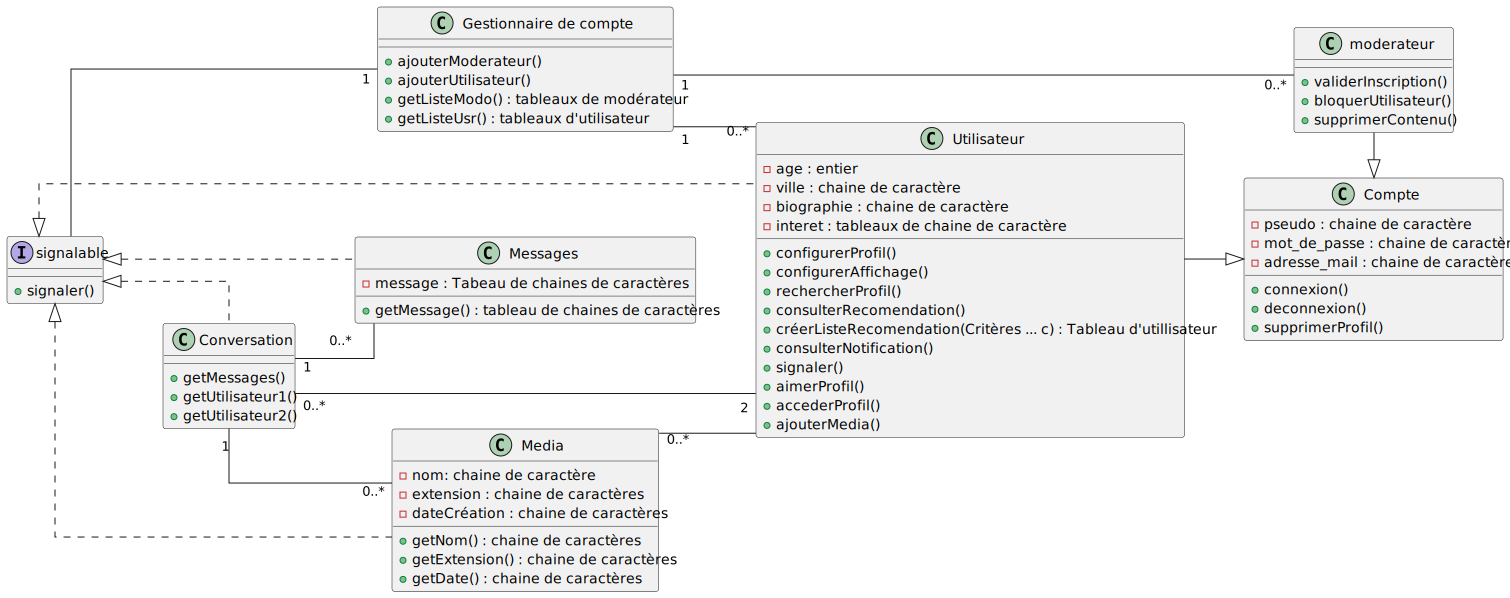
\includegraphics[width=\textwidth]{diag20.pdf}
	    \caption{Diagramme de classe}
	    \label{fig:diag20}
	\end{figure}
	
	
	
	\section{Maquette de l'application}
	\begin{figure}[H]
	    \centering
	    \includegraphics[width=0.7\textwidth]{1.png}
	    \caption{Page d’accueil en cas de premier accès}
	    \label{fig:diag21}
	\end{figure}
	
	\begin{figure}[H]
	    \centering
	    \includegraphics[width=0.7\textwidth]{2.png}
	    \caption{Page de connexion}
	    \label{fig:diag22}
	\end{figure}
	
	\begin{figure}[H]
	    \centering
	    \includegraphics[width=0.7\textwidth]{3.png}
	    \caption{Page d'inscription}
	    \label{fig:diag23}
	\end{figure}
	
	\begin{figure}[H]
	    \centering
	    \includegraphics[width=0.7\textwidth]{4.png}
	    \caption{Page d’accueil}
	    \label{fig:diag24}
	\end{figure}
	
	\begin{figure}[H]
	    \centering
	    \includegraphics[width=0.7\textwidth]{5.png}
	    \caption{Page de recherche de profil}
	    \label{fig:diag25}
	\end{figure}
	
	\begin{figure}[H]
	    \centering
	    \includegraphics[width=0.7\textwidth]{6.png}
	    \caption{Page de conversations}
	    \label{fig:diag26}
	\end{figure}
	
	\begin{figure}[H]
	    \centering
	    \includegraphics[width=0.7\textwidth]{7.png}
	    \caption{Page de modification du profil public}
	    \label{fig:diag27}
	\end{figure}
	
	\begin{figure}[H]
	    \centering
	    \includegraphics[width=0.7\textwidth]{8.png}
	    \caption{Page de configuration du profil}
	    \label{fig:diag28}
	\end{figure}
	
	
	\section{Dictionnaire}
	\begin{figure}[H]
		\centering
		\includegraphics[width=\textwidth]{dico.pdf}
		\caption{Dictionnaire}
		\label{fig:diag29}
	\end{figure}
	
	\section{Schéma entité-association}
	\begin{figure}[H]
		\centering
		\includegraphics[width=\textwidth]{diagEA.pdf}
		\caption{Schéma entité association}
		\label{fig:diag30}
	\end{figure}
	

\end{document}